\section{Dynamic Pipeline Framework in Haskell}\label{dp-hs}
The design and implementation of \acrfull{dpfh} is a fundamental piece of the present work. 
A \acrlong{dpf} written in \acrlong{hs} which allow \acrshort{hs} users to implement any suitable algorithm for \acrlong{dp}.
During the process of conducting this research, we have implemented \acrshort{dpfh}~\cite{dynamic-pipeline} and publishes it into \acrlong{hack}~\cite{hackage}.
In this section, we describe the design and implementation details of \acrshort{dpfh}.

\subsection{Framework Design}

\subsubsection{Background}
A suitable framework should provide the user the right level of abstraction that removes and hides underlying complexity, 
allowing the developer to focus on the problem that needs to be solved.
There are several design approximations to implement a framework: \begin{inparaenum}[i\upshape)]
  \item  \emph{Configuration Based} where the user only focuses on completing a specific configuration either on a file or a database or both. Once this configuration is completed, the user provides it to the framework's runtime system in order to execute the program. An example of this could be WordPress~\cite{wordpress},
  \item  \emph{Convention over Configuration (CoC)} where the user writes his code and definition following certain patterns in naming or source code location. Using the source code and content-specific information, the framework interprets the execution flow that needs to be executed. This technique has been deeply explored in the last $10$ years. One of the first framework that introduce this design paradigm was Ruby on Rails~\cite{rubyonrails}. Other examples are Spring Boot and Cake PHP for example \cite{springboot, cakephp},
  \item \emph{Application Programing Interface (API)} where the framework or library provides a certain amount of functionality implemented in terms of functions or interfaces, and the user needs to compose those functions or implement those abstractions to achieve the desired results. This has been the traditional design paradigm for building any library or framework, and finally
  \item \emph{\acrfull{dsl}}~\cite{Fowler10} where the framework or library provides a new language that represents the domain problem, encoding the solution in terms of that \acrshort{dsl} language. An example of this type of design is Hibernate Query Language~\cite{hql}
   \end{inparaenum}.

There exists two types of \acrlong{dsl}s~\cite{dsl}: External \acrfull{dsl} and \acrfull{edsl}. The purpose of \acrshort{dsl}, is to create a completely new language with its own semantic, syntax, and interpreter. 
\acrshort{dsl}s are not general-purpose languages, because as their name indicates, they are domain-specific. \acrshort{edsl} are syntactically embedded in the host language of the library, and the user writes in that host language, but restricted by the \acrshort{edsl} abstractions.
\acrshort{dpfh} follows a \acrshort{edsl} approach taking advantage of the strong type \acrshort{hs} system providing correctness at type-level~\cite{curryhoward}.

\subsubsection{Architectural Design}
In this section we focus on the architectural design of the \acrshort{dpfh} using a \acrshort{edsl} approach. We have built a framework that contains
three important components: \acrshort{dsl}, \acrshort{idl} and \acrshort{rs}. 

\begin{figure}[!ht]
  \centering
   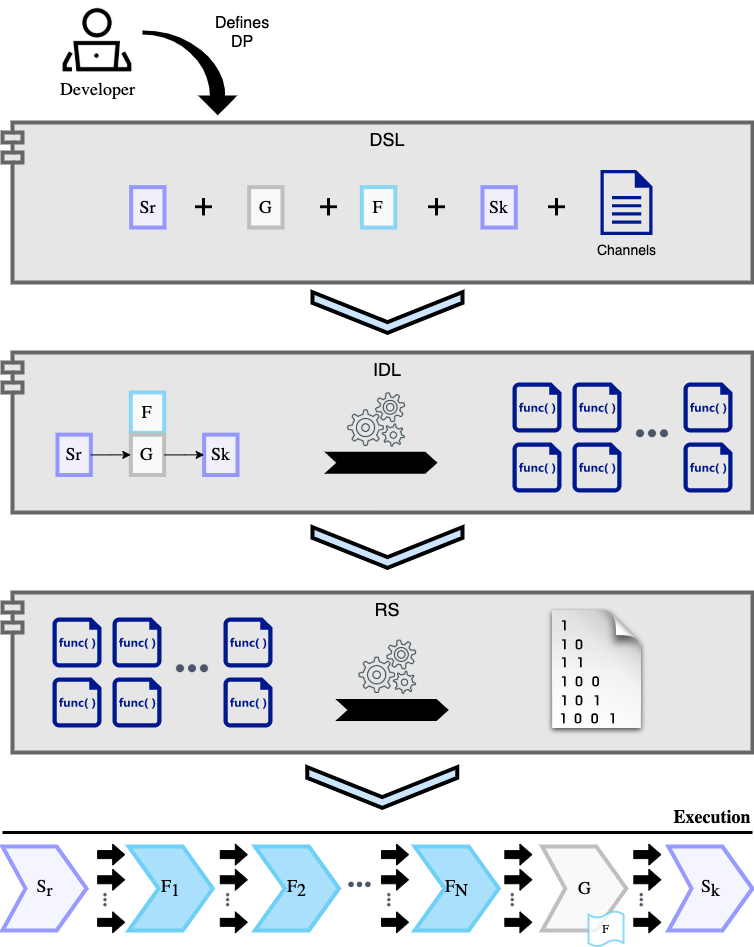
\includegraphics[width=1\textwidth, height=0.6\textheight]{dpf_haskell_v3.png}
    \caption[{[\acrshort{dpfh}] Architectural design of \acrshort{dpfh}}]{This diagram shows the architectural design of \acrshort{dpfh}. \acrshort{dpfh} is a \acrshort{dsl} which is built on three main components: \acrshort{dsl}, \acrshort{idl} and \acrshort{rs}. In the \acrshort{dsl} we can see how the user can compose the main stages of the \acrshort{dp}. \acrshort{idl} is showing how the frameworks is helping the user to transform that definition into real function or computations. Finally \acrshort{rs} execute all that definition plus functions. Execution layer indicates an example of a \acrshort{dp} running after being executed.}
    \label{fig:dpfh:1}
\end{figure}

In \autoref{fig:dpfh:1} we can appreciate the different components mentioned before that are the grey boxes.

\paragraph{DSL} The user interacts with the \acrshort{dsl} component where defines how the \acrshort{dp} flow
should be. Defining the flow consists on to provide a type-level specification about the channels that communicate each stage of the pipeline, as well as the data types those channels carry. 
For example, in the case of \autoref{prole} that we develop the \acrshort{wcc} algorithm, the user knows stages $\iwcc$, $\gwcc$, and $\owcc$ need to be connected with two channels. 
One of those channels is carrying the edges -- \texttt{Edge} data type -- and the other the accumulated connected components -- \texttt{ConnectedComp} data type --. 

\paragraph{IDL} Based on the definition provided in the \acrshort{dsl}, the user interacts with the \acrshort{idl} to build the functions with the algorithms needed for each stage: $\iwcc$, $\gwcc$, $\owcc$, $\fwcc$, and actors. 

\paragraph{RS} \acrshort{rs} is fed with the \acrshort{dp} definition and the functions implementations to finally execute the program. 

\subsection{Implementation}
In this section, we describe the implementation details of each architectural layer: \acrshort{dsl}, \acrshort{idl} and \acrshort{rs}.
As we have explained in \autoref{sec:contrib}, this library was published on Hackage~\cite{dynamic-pipeline}, the source code is open and can be found on this Github Repository~\cite{dynamic-pipeline-git}.

\subsubsection{DSL Grammar}\label{sub:sec:dsl-gram}
In order to provide correctness verification at compilation level, we define a \acrfull{cfg} that generates a \acrshort{dp} \acrshort{dsl} language. 
\acrshort{cfg} enables the user to define a \acrshort{dp} at type-level. 

\begin{definition}[\acrshort{dsl} \acrshort{cfg}]\label{def:cfg:dsl}
Lets $\gdsl = (N, \Sigma, DB, P)$ be a Context-Free Grammar, such that $N$ is the set of non-terminal symbols, $\Sigma$ the set of terminal symbols,
$DP \in N$ is the start symbol and $P$ are the generation rules. \autoref{fig:def:dpfh:dsl} shows the formal definition of the grammar.
\begin{figure}[H]
\begin{equation*}
    \boxed{
      \begin{aligned}
    N &= \{DP,S_r,S_k,G,F_b,CH,CH_s\},\\
    \Sigma &= \{\text{\mintinline{haskell}{Source}},\text{\mintinline{haskell}{Generator}},\text{\mintinline{haskell}{Sink}},\text{\mintinline{haskell}{FeedbackChannel}},\text{\mintinline{haskell}{Type}},\text{\mintinline{haskell}{Eof}},\text{\mintinline{haskell}{:=>}},\text{\mintinline{haskell}{:<+>}}\},
    \end{aligned}
    }
\end{equation*}
\begin{equation*}
  \boxed{
    \begin{aligned}
  P = \{\\
  DP  &\rightarrow S_r\ \text{\mintinline{haskell}{:=>}}\ G\ \text{\mintinline{haskell}{:=>}}\ S_k\ |\ S_r\ \text{\mintinline{haskell}{:=>}}\ G\ \text{\mintinline{haskell}{:=>}}\ F_b\ \text{\mintinline{haskell}{:=>}}\ S_k,\\
  S_r &\rightarrow \text{\mintinline{haskell}{Source}}\ CH_s,\\
  G   &\rightarrow \text{\mintinline{haskell}{Generator}}\ CH_s,\\
  S_k &\rightarrow \text{\mintinline{haskell}{Sink}},\\
  F_b &\rightarrow \text{\mintinline{haskell}{FeedbackChannel}} CH,\\
  CH_s &\rightarrow \text{\mintinline{haskell}{Channel}}\ CH,\\
  CH &\rightarrow \text{\mintinline{haskell}{Type :<+>}}\ CH\ |\ \text{\mintinline{haskell}{Eof}}\}
\end{aligned}
}
\end{equation*}
\caption[{[\acrshort{dpfh}] DSL Grammar definition}]{This is the Context-Free Grammar defined for the DSL. In the first box we can see $N$ which is the set of non-terminals symbols of the Grammar. $\Sigma$ which is the set of the terminal symbols and $P$ the production rules of the grammar.}
\label{fig:def:dpfh:dsl}
\end{figure}
\end{definition}

For encoding $\gdsl$ on the \acrshort{hs}, we use an \emph{Index type}~\cite{type-index} to keep track, at type-level, of the extra information required by the \acrshort{dp} definition such as channels and data types the channels carry. 

\begin{listing}[H]
  \begin{minted}[fontsize=\fontsize{10}{11}\selectfont,numbers=left,breaklines,frame=lines,framerule=2pt,framesep=2mm,baselinestretch=1.2,highlightlines={3,4}]{haskell}

data Source (a :: Type)
data Generator (a :: Type)
data Sink
data Eof
data Channel (a :: Type)
data FeedbackChannel (a :: Type)

  \end{minted}
  \caption[{[\mintinline{shell}{Flow.hs}] $\Sigma$ enconding of $G_{dsl}$}]{This code is showing most of the data types that represent the same terminal symbols $\Sigma \in G_{dsl}$. Those types that are indexed by another kind \mintinline{haskell}{Type}, allows to store information at type-level needed for interpret the DSL}
  \label{src:dpfh:1}
\end{listing}
  
In \autoref{src:dpfh:1}, there is an \emph{Index type} for each element of $\Sigma$ encoded in \acrshort{hs} Types.
The highlighted lines in \autoref{src:dpfh:1} shows the terminal symbols $\Sigma$ that are not indexed, because neither \mintinline{haskell}{Sink} nor \mintinline{haskell}{Eof} are carrying extra type-level information. 
In the case of \mintinline{haskell}{Sink}, since it is the last stage that does not connect further with any other stage, we do not need to indicate any channel information. 
\mintinline{haskell}{Eof} it is just a terminal type to disambiguate the \mintinline{haskell}{Channel (a :: Type)} subtree for the full parser tree. 
\mintinline{haskell}{Channel} can carry any type because it needs to be polymorphic to support a different number of channels and data types.

\begin{listing}[H]
  \begin{minted}[fontsize=\fontsize{10}{11}\selectfont,numbers=left,breaklines,frame=lines,framerule=2pt,framesep=2mm,baselinestretch=1.2,highlightlines={1,5}]{haskell}
    
    data chann1 :<+> chann2 = chann1 :<+> chann2
    deriving (Typeable, Eq, Show, Functor, Traversable, Foldable, Bounded)
    infixr 5 :<+>
    
    data a :=> b = a :=> b
    deriving (Typeable, Eq, Show, Functor, Traversable, Foldable, Bounded)
    infixr 5 :=>
    
  \end{minted}
  \caption[{[\mintinline{shell}{Flow.hs}] $\Sigma$ enconding of $G_{dsl}$ - Especial non-terminals}]{Special terminal symbols $\{\text{\mintinline{haskell}{:<+>}}, \text{\mintinline{haskell}{:=>}}\} \in \Sigma$. This terminal symbols allows to index two types in order to combine several of them and build a chain of stages (\mintinline{haskell}{:=>}) and a set of channels (\mintinline{haskell}{:<+>}).}
  \label{src:dpfh:2}
\end{listing}

There are two important terminal symbols in $\Sigma$: \mintinline{haskell}{:=>} and \mintinline{haskell}{:<+>}.
In \autoref{src:dpfh:2}, the definition shows how \mintinline{haskell}{:=>} and \mintinline{haskell}{:<+>} can combine 2 (two) types. 
The propose of writing \mintinline{haskell}{:=>} and \mintinline{haskell}{:<+>} as types is to have a syntactic sugar type combinator for writing the \acrshort{dsl} according to the \acrshort{cfg}. 
Apart from that, they are different because two distinguishable terminal symbols $\Sigma$ are needed to separate the encoding of the pipeline stage ($\iwcc$, $\gwcc$, $\owcc$)
from the encoding of channel composition in the same stage, as we can appreciate in \dref{def:cfg:dsl}.

Now, we can start defining our pipelines at type-level. For example, if we want to generate a \acrshort{dp} that eliminates duplicated elements in a stream, we know that we only need one channel connecting the stages that carries out the type of the element, in this case, \mintinline{haskell}{Int} (see \autoref{src:dpfh:3}).

\begin{listing}[H]
  \begin{minted}[fontsize=\fontsize{10}{11}\selectfont,numbers=left,breaklines,frame=lines,framerule=2pt,framesep=2mm,baselinestretch=1.2,highlightlines={}]{haskell}

type DPExample = Source (Channel (Int :<+> Eof)) 
              :=> Generator (Channel (Int :<+> Eof)) 
              :=> Sink
   
  \end{minted}
  \caption[{[\mintinline{shell}{Repeated.hs} Example of \acrshort{dp} encoded in $G_{dsl}$}]{This example shows the \acrshort{dsl} encoding in \acrshort{dp} of repeated elements problems}
  \label{src:dpfh:3}
\end{listing}

\subsubsection{DSL Validation}\label{sub:sec:dsl-val}
The language generated by the grammar needs to be validated to avoid errors or provide an incorrect \acrshort{dp} definition.
Fortunately, \acrshort{hs} provides several Type-level techniques~\cite{type-haskell} which allows to verify properties of programs before running them, 
preventing the users to introduce bugs, reducing errors. This verification done by the compiler establish a Curry-Howard Isomorphism~\cite{curryhoward}, i.e. 
\emph{Propositions as Types - Programs as Proof}. It is important to remark here that \acrshort{hs} is not a theorem prover System like Coq~\cite{coq}, but some verifications, as we present in this work, can be done with \acrshort{ghc} to ensure correctness on programs.
Although \acrshort{hs} provides tools to build advanced type-level verifications, all these techniques require the addition of \emph{Haskell Language Extensions}.

Once we have the encoded \acrshort{dp} problem in the \acrshort{dsl} grammar -- see \autoref{sub:sec:dsl-gram} --, we can proceed on validating that encoded grammar. 
The implementation of the validation of the \acrshort{dsl} \acrshort{cfg} at type-level, has been done using \emph{Associated Type Families}~\cite{associated-types}.

\begin{listing}[H]
  \begin{minted}[fontsize=\fontsize{10}{11}\selectfont,numbers=left,breaklines,frame=lines,framerule=2pt,framesep=2mm,baselinestretch=1.2,highlightlines={6,18}]{haskell}

type family And (a :: Bool) (b :: Bool) :: Bool where
    And 'True 'True = 'True
    And a b         = 'False
  

type family IsDP (dpDefinition :: k) :: Bool where
    IsDP (Source (Channel inToGen) :=> Generator (Channel genToOut) :=> Sink)
        = And (IsDP (Source (Channel inToGen))) (IsDP (Generator (Channel genToOut)))
    IsDP ( Source (Channel inToGen) :=> Generator (Channel genToOut) :=> FeedbackChannel toSource :=> Sink)
        = And (IsDP (Source (Channel inToGen))) (IsDP (Generator (Channel genToOut)))
    IsDP (Source (Channel (a :<+> more)))     
        = IsDP (Source (Channel more))
    IsDP (Source (Channel Eof))               = 'True
    IsDP (Generator (Channel (a :<+> more)))  = IsDP (Generator (Channel more))
    IsDP (Generator (Channel a))              = 'True
    IsDP x                                    = 'False
     
type family ValidDP (a :: Bool) :: Constraint where
  ValidDP 'True = ()
  ValidDP 'False = TypeError
                    ( 'Text "Invalid Semantic for Building DP Program"
                      ':$$: 'Text "Language Grammar:"
                      ':$$: 'Text "DP       -> Source CHANS :=> Generator CHANS :=> Sink"
                      ':$$: 'Text "DP       -> Source CHANS :=> Generator CHANS :=> FEEDBACK :=> Sink"
                      ':$$: 'Text "CHANS    -> Channel CH"
                      ':$$: 'Text "FEEDBACK -> FeedbackChannel CH"
                      ':$$: 'Text "CH       -> Type :<+> CH | Eof"
                      ':$$: 'Text "Example: 'Source (Channel (Int :<+> Int)) :=> Generator (Channel (Int :<+> Int)) :=> Sink'"
                    )
  \end{minted}
  \caption[{[\mintinline{shell}{Stage.hs}] Validating encoded in $G_{dsl}$ - FCF}]{Type Families \mintinline{haskell}{And}, \mintinline{haskell}{IsDP} and \mintinline{haskell}{ValidDP} which allows to perform a type-level validation over a \acrshort{dsl} \acrshort{cfg} definition.}
  \label{src:dpfh:4}
\end{listing}

In \autoref{src:dpfh:4}, there are 3(three) Type families that helps to validate the \acrshort{dsl} \acrshort{cfg}. 
\mintinline{haskell}{IsDP} associated type family is checking the production rules $P$ of the grammar defined in \autoref{fig:def:dpfh:dsl}, returning a promoted data type~\cite{promoted-types} (not a boolean value) \mintinline{haskell}{'True} in case
the production rule matches all the generated language, or \mintinline{haskell}{'False} otherwise. 
\mintinline{haskell}{ValidDP} is taking the result of \mintinline{haskell}{IsDP} type application, associating \mintinline{haskell}{'True} promoted boolean type to empty \mintinline{haskell}{()} constraint. An empty constraint is an 
indication of nothing to be restricted, meaning that if \mintinline{haskell}{ValidDP} is used as a constraint, and it is fully applied to \mintinline{haskell}{()}, it will give the compiler the evidence that there is no error at type-level.
\mintinline{haskell}{ValidDP} is also associating \mintinline{haskell}{'False} to a custom \mintinline{haskell}{TypeError} which will appear at compilation time if the \acrshort{dp} \acrshort{dsl} definition fully applies to that.

\begin{listing}[H]
  \begin{minted}[fontsize=\fontsize{10}{11}\selectfont,numbers=left,breaklines,frame=lines,framerule=2pt,framesep=2mm,baselinestretch=1.2,highlightlines={2}]{haskell}

mkDP :: forall dpDefinition filterState filterParam st.
    ( ValidDP (IsDP dpDefinition)
    , DPConstraint dpDefinition filterState st filterParam)
 => Stage (WithSource dpDefinition (DP st)) 
 -> GeneratorStage dpDefinition filterState filterParam st  
 -> Stage (WithSink dpDefinition (DP st))  
 -> DP st ()
mkDP = ...

someFunc = mkDP @DPExample ...

  \end{minted}
  \caption[{[\mintinline{shell}{Stage.hs}] Using validation of \acrshort{dp} encoded in $G_{dsl}$}]{Definition of \mintinline{haskell}{mkDP} function of the Framework which uses type-level validation of the grammar \mintinline{haskell}{ValidDP (IsValid Type)}. Last line of the code is showing that using that function will compile-time check the definition of \mintinline{haskell}{DPExample} type.}
  \label{src:dpfh:5}
\end{listing}

\subsubsection{\acrfull{idl}}
\acrshort{idl} component takes the \acrshort{dp} definition made on with \acrshort{dsl} component to interpret and generate the function definitions
that the user needs to fill in for solving a specific problem. In \autoref{sec:dp}, we have described what the user needs to provide in a \acrshort{dp} algorithm: $\iwcc$, $\gwcc$, $\owcc$, and the $\fwcc$ with the non-empty set of Actors.
The \acrshort{idl} generates the function definitions with an empty implementation to be completed by the user, ensuring that those functions will give "Proof" -- in terms of Curry-Howard Correspondence~\cite{curryhoward} --  of the "Propositions" defined on the \acrshort{dsl}.

Similar techniques that we used on \autoref{sub:sec:dsl-val} are also used here. 
On the first hand, we use \emph{Type-level Defunctionalization}~\cite{defunctionalization, fun-type-function-haskell} to let the compiler generates the signatures of the required functions. 
On the other hand, we use \emph{Term-level Defunctionalization} to interpret those functions.
Moreover, \emph{Indexed Types}~\cite{type-index} and \emph{Heterogeneous List}~\cite{hlist} are used to keep track of the dynamic number and polymorphic types of the functions parameters. 

\begin{listing}[H]
  \begin{minted}[fontsize=\fontsize{10}{11}\selectfont,numbers=left,breaklines,frame=lines,framerule=2pt,framesep=2mm,baselinestretch=1.2,highlightlines={2,6,10}]{haskell}
withSource :: forall (dpDefinition :: Type) st. WithSource dpDefinition (DP st) 
            -> Stage (WithSource dpDefinition (DP st))
withSource = mkStage' @(WithSource dpDefinition (DP st))

withGenerator :: forall (dpDefinition :: Type) (filter :: Type) st. WithGenerator dpDefinition filter (DP st) 
              -> Stage (WithGenerator dpDefinition filter (DP st))
withGenerator = mkStage' @(WithGenerator dpDefinition filter (DP st))

withSink :: forall (dpDefinition :: Type) st. WithSink dpDefinition (DP st) 
           -> Stage (WithSink dpDefinition (DP st))
withSink = mkStage' @(WithSink dpDefinition (DP st))
  \end{minted}
  \caption[{[\mintinline{shell}{Stage.hs}] Using with Interpreters of \acrshort{dp} encoded in $G_{dsl}$}]{This code is showing the different interpreters combinators to help the user to generate the functions of the principal stages of \acrshort{dp}}
  \label{src:dpfh:6}
\end{listing}

In \autoref{src:dpfh:6} we can appreciate the different combinators of the \acrshort{idl} that helps the user of the framework to interpret the \acrshort{dsl} to generate the function definitions.
\mintinline{haskell}{Stage} data type will be cover in \autoref{src:dpfh:8}, but it is a wrapper type of a pipeline stage -- minimal unit of execution --, containing the function to be executed -- here is the use \emph{Term-level Defunctionalization} --.
\mintinline{haskell}{withSource}, \mintinline{haskell}{withGenerator}, and \mintinline{haskell}{withSink} are aliases of the function \mintinline{haskell}{mkStage'} which is the combinator that is applying the \emph{Associated Type} related to that stage. For example \mintinline{haskell}{withSource}, is equivalent to \mintinline{haskell}{mkStage' @(WithSource dpDefinition (DP st))}.
For each \emph{Associated Type Family} defintion, there exist an equivalent term-level definition: \mintinline{haskell}{WithSource} type with \mintinline{haskell}{withSource} term , \mintinline{haskell}{WithGenerator} type with \mintinline{haskell}{withGenerator} term, and \mintinline{haskell}{WithSink} type with \mintinline{haskell}{withSink} term -- notice the capital case letter "W" indicating the type and not the term --.

\begin{listing}[H]
  \begin{minted}[fontsize=\fontsize{10}{11}\selectfont,numbers=left,breaklines,frame=lines,framerule=2pt,framesep=2mm,baselinestretch=1.2,highlightlines={7,11}]{haskell}
type family WithSource (dpDefinition :: Type) (monadicAction :: Type -> Type) :: Type where
  WithSource (Source (Channel inToGen) :=> Generator (Channel genToOut) :=> Sink) monadicAction
      = WithSource (ChanIn inToGen) monadicAction
  WithSource (Source (Channel inToGen) :=> Generator (Channel genToOut) :=> FeedbackChannel toSource :=> Sink) monadicAction 
      = WithSource (ChanOutIn toSource inToGen) monadicAction
  WithSource (ChanIn (dpDefinition :<+> more)) monadicAction         
      = WriteChannel dpDefinition -> WithSource (ChanIn more) monadicAction
  WithSource (ChanIn Eof) monadicAction                              
      = monadicAction ()
  WithSource (ChanOutIn (dpDefinition :<+> more) ins) monadicAction  
      = ReadChannel dpDefinition -> WithSource (ChanOutIn more ins) monadicAction
  WithSource (ChanOutIn Eof ins) monadicAction                       
      = WithSource (ChanIn ins) monadicAction
  WithSource dpDefinition _                                          
      = TypeError
          ( 'Text "Invalid Semantic for Source Stage"
            ':$$: 'Text "in the DP Definition '"
            ':<>: 'ShowType dpDefinition
            ':<>: 'Text "'"
            ':$$: 'Text "Language Grammar:"
            ':$$: 'Text "DP       -> Source CHANS :=> Generator CHANS :=> Sink"
            ':$$: 'Text "DP       -> Source CHANS :=> Generator CHANS :=> FEEDBACK :=> Sink"
            ':$$: 'Text "CHANS    -> Channel CH"
            ':$$: 'Text "FEEDBACK -> FeedbackChannel CH"
            ':$$: 'Text "CH       -> Type :<+> CH | Eof"
            ':$$: 'Text "Example: 'Source (Channel (Int :<+> Int)) :=> Generator (Channel (Int :<+> Int)) :=> Sink'"
          )
  \end{minted}
  \caption[{[\mintinline{shell}{Stage.hs}] WithSource Associate Type Details}]{An example of the Associated Type Family \mintinline{haskell}{WithSource} that allows to implement \emph{Type-level Defunctionalization} technique that will be the Type-level verification of the term \mintinline{haskell}{withSource}}
  \label{src:dpfh:7}
\end{listing}

In \autoref{src:dpfh:7}, in the highlighted lines, it can be seen how \emph{Type-level Defunctionalization} is being expanded in a signature function definition with the form \mintinline{haskell}{WriteChannel a -> ReadChannel b -> ... -> monadicAction ()} depending on \acrshort{dp} language definition. 

\begin{listing}[H]
  \begin{minted}[fontsize=\fontsize{10}{11}\selectfont,numbers=left,breaklines,frame=lines,framerule=2pt,framesep=2mm,baselinestretch=1.2,highlightlines={12,16}]{haskell}

data Stage a where
  Stage :: Proxy a -> a -> Stage a

mkStage' :: forall a. a -> Stage a
mkStage' = Stage (Proxy @a)
    
  \end{minted}
  \caption[{[\mintinline{shell}{Stage.hs}] Stage Data Type}]{\mintinline{haskell}{Stage} data type for implementing \emph{Term-level Defunctionalization} providing evidence to the Type-Level Associated types}
  \label{src:dpfh:8}
\end{listing}

In \autoref{src:dpfh:8}, \mintinline{haskell}{Stage} data type uses a \mintinline{haskell}{Proxy} phantom type. 
This phantom type allow \mintinline{haskell}{Stage} to index the type definition generated by \mintinline{haskell}{a}.
For example, in \autoref{src:dpfh:6}, when \mintinline{haskell}{withSource} interpreter is applied to \mintinline{haskell}{WithSource dpDefinition},  
the compiler is provided with \mintinline{haskell}{dpDefinition} \acrshort{dsl} type, it expands the function signature belonging to that \acrshort{dp} definition inside the \mintinline{haskell}{Stage}.

\paragraph{Generator and Filter}
According to \acrshort{dp} definition in \autoref{sec:dp}, $\gwcc$ has a $\fwcc$ template in order to know how to dynamically interpose a new $\fwcc$ during the runtime execution of the program.
Let's first study $\fwcc$ Data Type in the context of the framework.

\begin{listing}[H]
  \begin{minted}[fontsize=\fontsize{10}{11}\selectfont,numbers=left,breaklines,frame=lines,framerule=2pt,framesep=2mm,baselinestretch=1.2,highlightlines={2,5}]{haskell}

newtype Actor dpDefinition filterState filterParam monadicAction =
    Actor {  unActor :: MonadState filterState monadicAction => Stage (WithFilter dpDefinition filterParam monadicAction) }

newtype Filter dpDefinition filterState filterParam st =
    Filter { unFilter :: NonEmpty (Actor dpDefinition filterState filterParam (StateT filterState (DP st))) }
    deriving Generic
    
  \end{minted}
  \caption[{[\mintinline{shell}{Stage.hs}] Filter / Actor Data Type}]{This code shows the definition of the \mintinline{haskell}{Filter} data type which contains a non-empty set of \mintinline{haskell}{Actor}. The \mintinline{haskell}{Actor} data type is an \mintinline{haskell}{Stage} in the Context of the \mintinline{haskell}{MonadState} to allow keeping a local memory in the execution context of the filter.}
  \label{src:dpfh:9}
\end{listing}

In \autoref{src:dpfh:9} the definition of the \mintinline{haskell}{Filter} data type contains a non-empty set of \mintinline{haskell}{Actor}.
An \mintinline{haskell}{Actor} is a \mintinline{haskell}{Stage}, because an actor is the minimal unit of execution of a filter. 
A \mintinline{haskell}{Filter} has a \mintinline{haskell}{NonEmpty Actor} -- Non-empty List -- because a filter is built by a sequence of actors calls. 
Moreover, \mintinline{haskell}{Actor} Stage is defunctionalized with \mintinline{haskell}{WithFilter} \emph{Associated Type Family}. 
\mintinline{haskell}{Filter} runs in an explicit \mintinline{haskell}{StateT} monadic context. This is because the $\fwcc$ instance should have an state, according to \acrshort{dp} definition in \autoref{sec:dp}.
For example, in the case of $\dpwcc$, as we have seen in \autoref{prole}, $\fwcc$ keeps an updated list of connected components that updates as long as it receives more edges that are connected with the current list of vertices.
\mintinline{haskell}{Actor} data type -- see \autoref{src:dpfh:9} --, is constrained by \mintinline{haskell}{MonadState} which is in the same execution context of the whole \mintinline{haskell}{NonEmpty Actor} list of the \mintinline{haskell}{Filter}. 
This means the \mintinline{haskell}{StateT} is executed for each \mintinline{haskell}{Actor} of that filter, sharing the same state between them. 

\begin{listing}[H]
  \begin{minted}[fontsize=\fontsize{10}{11}\selectfont,numbers=left,breaklines,frame=lines,framerule=2pt,framesep=2mm,baselinestretch=1.2,highlightlines={}]{haskell}

mkFilter :: forall dpDefinition filterState filterParam st. WithFilter dpDefinition filterParam (StateT filterState (DP st)) 
         -> Filter dpDefinition filterState filterParam st
mkFilter = Filter . single

single :: forall dpDefinition filterState filterParam st. WithFilter dpDefinition filterParam (StateT filterState (DP st)) 
       -> NonEmpty (Actor dpDefinition filterState filterParam (StateT filterState (DP st)))
single = one . actor

actor :: forall dpDefinition filterState filterParam st. WithFilter dpDefinition filterParam (StateT filterState (DP st)) 
      -> Actor dpDefinition filterState filterParam (StateT filterState (DP st))
actor = Actor . mkStage' @(WithFilter dpDefinition filterParam (StateT filterState (DP st)))

(|>>>) :: forall dpDefinition filterState filterParam st. Actor dpDefinition filterState filterParam (StateT filterState (DP st)) 
       -> Filter dpDefinition filterState filterParam st 
       -> Filter dpDefinition filterState filterParam st
(|>>>) a f = f & _Wrapped' %~ (a <|)
infixr 5 |>>>

(|>>) :: forall dpDefinition filterState filterParam st. Actor dpDefinition filterState filterParam (StateT filterState (DP st)) 
      -> Actor dpDefinition filterState filterParam (StateT filterState (DP st)) 
      -> Filter dpDefinition filterState filterParam st
(|>>) a1 a2 = Filter (a1 <|one a2)
infixr 5 |>>
  \end{minted}
  \caption[{[\mintinline{shell}{Stage.hs}] Filter / Actor smart constructors and combinators}]{Combinators and small constructor to enable building actors and filter.}
  \label{src:dpfh:10}
\end{listing}

Finally, in \autoref{src:dpfh:10}, some combinators and smart constructors are provided in the framework to enable the construction of \mintinline{haskell}{Filter} and \mintinline{haskell}{Actor}.
\mintinline{haskell}{mkFilter} is a smart constructor for \mintinline{haskell}{Filter} Data Constructor. \mintinline{haskell}{single} wraps one actor inside a \mintinline{haskell}{Filter}.
\mintinline{haskell}{actor} is a smart constructor for \mintinline{haskell}{Actor} Data Constructor. \mintinline{haskell}{(|>>>)} is an appending combinator of an \mintinline{haskell}{Actor} to a \mintinline{haskell}{Filter}. 
\mintinline{haskell}{(|>>>)} also ensures actor execution order, i.e. the latest actor added is the latest to be executed.


\begin{listing}[H]
  \begin{minted}[fontsize=\fontsize{10}{11}\selectfont,numbers=left,breaklines,frame=lines,framerule=2pt,framesep=2mm,baselinestretch=1.2,highlightlines={}]{haskell}
    data GeneratorStage dpDefinition filterState filterParam st = GeneratorStage
    { _gsGenerator      :: Stage (WithGenerator dpDefinition (Filter dpDefinition filterState filterParam st) (DP st))
    , _gsFilterTemplate :: Filter dpDefinition filterState filterParam st
    }  
  \end{minted}
  \caption[{[\mintinline{shell}{Stage.hs}] Generator}]{\mintinline{haskell}{Generator} Data type which contains the \mintinline{haskell}{Stage} code of the generator itself, and the \mintinline{haskell}{Filter} template that it can be spawned by the \mintinline{haskell}{Generator}.}
  \label{src:dpfh:11}
\end{listing}

In \autoref{src:dpfh:11}, $\gwcc$ contains a $\fwcc$ template and its own stage behavior.
\mintinline{haskell}{Generator} data type has a field with the \mintinline{haskell}{Filter} template that could be spawned by the algorithm defined by the user according to the data received from its input channels.
\mintinline{haskell}{Generator} has also another field with the behavior of the $\gwcc$ -- a \mintinline{haskell}{Stage} --. 

\subsubsection{\acrfull{rs}}
The \acrshort{rs} can be divided into two parts: the mechanism to generate stages dynamically in runtime, and the execution entry point of the \acrshort{dp}.
Regarding execution entry point, all the stages that we have seen in previous sections are the pieces needed to build an executable \mintinline{haskell}{DP st a} monad.
This executable monad has an existential type similar to \mintinline{haskell}{ST} monad to not escape out from the context on different stages.
Once the dynamic pipeline starts to execute, the core of the framework dynamically generates stages between $\gwcc$ and previous stages, according to the user definition, i.e. an \emph{anamorphism}~\cite{lenses} that creates $\fwcc$ instances until some condition is met.

\begin{listing}[H]
  \begin{minted}[fontsize=\fontsize{10}{11}\selectfont,numbers=left,breaklines,frame=lines,framerule=2pt,framesep=2mm,baselinestretch=1.2,highlightlines={2,12,14,15,16,17,18}]{haskell}
unfoldF :: forall dpDefinition readElem st filterState filterParam l. SpawnFilterConstraint dpDefinition readElem st filterState filterParam l
        => UnFoldFilter dpDefinition readElem st filterState filterParam l 
        -> DP st (HList l) 
unfoldF = loopSpawn

where
  loopSpawn uf@UnFoldFilter{..} =
    maybe (pure _ufRsChannels) (loopSpawn <=< doOnElem uf) =<< DP (pull _ufReadChannel)

  doOnElem uf@UnFoldFilter{..} elem' = do
    _ufOnElem elem'
    if _ufSpawnIf elem'
     then do
       (reads', writes' :: HList l3) <- getFilterChannels <$> DP (makeChansF @(ChansFilter dpDefinition))
       let hlist = elem' .*. _ufReadChannel .*. (_ufRsChannels `hAppendList` writes')
       void $ runFilter _ufFilter (_ufInitState elem') hlist (_ufReadChannel .*. (_ufRsChannels `hAppendList` writes'))
       return $ uf { _ufReadChannel = hHead reads', _ufRsChannels = hTail reads' }
     else return uf

  \end{minted}
  \caption[{[\mintinline{shell}{Stage.hs}] unfoldF}]{\mintinline{haskell}{unfolF} is the \emph{anamorphism} combinator to spawn new \mintinline{haskell}{Filter} types between the \mintinline{haskell}{Generator} and previous stages.}
  \label{src:dpfh:12}
\end{listing}

In \autoref{src:dpfh:12}, it is presented how is the \emph{anamorphism} mechanims that generates dynamic stages between $\gwcc$ and the previous stages.
That \emph{anamorphism} is implemented with the function \mintinline{haskell}{unfoldF}. That function receives an \mintinline{haskell}{UnFoldFilter} Data type, which contains the recipe for controlling that unfold recursive call. 
In line $12$, \mintinline{haskell}{_ufSpawnIf} field of \mintinline{haskell}{UnFoldFilter}, indicates when to stop the recursion. 
Inside the conditional, in line $14$, new channels are created for the new filter to be spawned. Those new channels connect the new filter with the previous stages and with \mintinline{haskell}{Generator}. 
After that, in line $16$ \mintinline{haskell}{runFilter} starts the monadic computation, spawning the filter stage with its actors.
Finally, the new list of channels are returned for the next recursive step to allow further channel connections.

\begin{listing}[H]
  \begin{minted}[fontsize=\fontsize{10}{11}\selectfont,numbers=left,breaklines,frame=lines,framerule=2pt,framesep=2mm,baselinestretch=1.2,highlightlines={}]{haskell}
mkUnfoldFilter :: (readElem -> Bool) 
    -> (readElem -> DP st ()) 
    -> Filter dpDefinition filterState filterParam st 
    -> (readElem -> filterState)
    -> ReadChannel readElem
    -> HList l 
    -> UnFoldFilter dpDefinition readElem st filterState filterParam l


mkUnfoldFilterForAll' :: (readElem -> DP st ())
                      -> Filter dpDefinition filterState filterParam st
                      -> (readElem -> filterState)
                      -> ReadChannel readElem
                      -> HList l
                      -> UnFoldFilter dpDefinition readElem st filterState filterParam l

mkUnfoldFilterForAll :: Filter dpDefinition filterState filterParam st
                      -> (readElem -> filterState)
                      -> ReadChannel readElem
                      -> HList l
                      -> UnFoldFilter dpDefinition readElem st filterState filterParam l
   \end{minted}
  \caption[{[\mintinline{shell}{Stage.hs}] UnfoldFilter combinators}]{Combinators for building \mintinline{haskell}{UnfoldFilter} types indicating the type of the \mintinline{haskell}{unfold} that the user want to achieve.}
  \label{src:dpfh:13}
\end{listing}

Several smart constructors are also provided for building \mintinline{haskell}{UnfoldFilter} Data Type.
In \autoref{src:dpfh:13} the first combinator is the default smart constructor.  \begin{inparaenum}[i\upshape)]
  \item First field \mintinline{haskell}{(readElem -> Bool)} indicate if the a new filter should be spawn or not.
  \item Second field \mintinline{haskell}{(readElem -> DP st ())} is a monadic optional computation to do when received a new element, for example logging.
  \item Third field \mintinline{haskell}{Filter} data type to be spawned.
  \item Fourth field \mintinline{haskell}{(readElem -> filterState)} is initialization of the \mintinline{haskell}{Filter} State.
  \item Fifth field \mintinline{haskell}{(ReadChannel readElem)} that feeds the filter instance.
  \item Last field is the \emph{Heterogeneous List} with the rest of the channels to connect with other stages.
\end{inparaenum}.
The combinator \mintinline{haskell}{mkUnfoldFilterForAll} is an smart constructor of \mintinline{haskell}{UnfoldFilter} that allows to spawn a new filter for each element received in the $\gwcc$.

\subsection{Libraries and Tools}
\subsection{Parallelization} 
One of the most important components of the implementation is the selection of concurrency libraries to support an intensive parallelization workload. Parallelization techniques and tools have been intensively studied and implemented in \acrshort{hs} \cite{monadpar}. 
Indeed, it is well known that green threads and sparks allow spawning thousands to millions of parallel computations. 
These parallel computations do not penalize performance when compare with \acrfull{os} level threading \cite{parallelbook}. 
A straightforward assumption to achieve here, is to use \texttt{monad-par} library \cite{monadparlib, monadpar}. 
Nevertheless, in this work, we have discarded the use of sparks \cite{sparks} because we can achieve the level of required parallelism spawning green threads only.
The next obvious choice is to use \mintinline{haskell}{forkIO :: IO () -> IO ThreadId} from \texttt{base} library \cite{forkio}. 
However, that would imply handling all the threads lifecycles and errors programmatically without any abstraction to facilitate that complex task. 
Therefore, we choose \texttt{async} library \cite{async} which enables to spawn asynchronous computations \cite{parallelbook} on \acrshort{hs} using green threads, and at the same time, it provides useful combinators to managing thread terminations and errors.

\subsubsection{Channels\label{section:channels}} 
We have several techniques to our disposal to communicate between threads or sparks in \acrshort{hs} like \mintinline{haskell}{MVar} or concurrent safe mechanisms like \acrfull{stm} \cite{stm}. 
At the same time, in \acrshort{hs} library ecosystem, we dispose of \texttt{Channels} abstractions based on both mentioned communication techniques. 
In that sense, for conducting the communication between dynamic stages and data flowing in a \acrshort{dp}, we have selected \texttt{unagi-chan} library \cite{unagi} which provides the following advantages to our solution: Firstly, \mintinline{haskell}{MVar} channel without using \acrshort{stm} reducing overhead. 
\acrshort{stm} is not required in a \acrshort{dp} because one specific stage which is running in a separated thread, can only access to its \texttt{I/O} channels for reading/writing accordingly, and those operations are not concurrently shared by other threads (stages) for the same channels. 
Second, non-blocking channels. \texttt{unagi-chan} library contains blocking and non-blocking channels for reading. This aspect is key to gain speed up on the implementation. Third, the library is optimized for $x86$ architectures with use of low-level \texttt{fetch-and-add} instructions. Finally, \texttt{unagi-chan} is $100x$ faster~\cite{unagi-bench} on Benchmarking compare with \acrshort{stm} and default base \mintinline{haskell}{Chan} implementations.

